\documentclass[a4paper,11pt,twoside]{book}
\usepackage{listings}		
\usepackage{graphicx}
\usepackage[svgnames]{xcolor}
\usepackage{multicol}
\usepackage{adjustbox}
\usepackage{amssymb} 
\usepackage{amsmath}
\usepackage[ruled,vlined]{algorithm2e}
\usepackage{hyperref}
\usepackage{mathtools}
\usepackage{nicefrac}
\usepackage[makeroom]{cancel}

% \DeclarePairedDelimiter{\ceil}{\lceil}{\rceil}
% \DeclarePairedDelimiter{\abracket}{\langle}{\rangle}
\hypersetup{
    colorlinks,
    citecolor=black,
    filecolor=black,
    linkcolor=black,
    urlcolor=black
}

\setlength{\tabcolsep}{1em}
\setlength{\emergencystretch}{10pt}
\graphicspath{ {./img/} }	
% \pagecolor{black}
% \color{white}				

\lstset{language=Java,						
	showspaces=false,
	showtabs=false,
	breaklines=true,
	showstringspaces=false,
	breakatwhitespace=true,
	commentstyle=\color{ForestGreen},
	keywordstyle=\color{blue},
	stringstyle=\color{red},
	identifierstyle=\color{Gray},
	basicstyle=\small\ttfamily
}

\newcommand{\bluetext}[1]{\textcolor{blue}{#1}}
\newcommand{\redtext}[1]{\textcolor{red}{#1}}
\newcommand{\orangetext}[1]{\textcolor{orange}{#1}}
\newcommand{\subtext}[1]{\textsubscript{#1}}
\newcommand{\supertext}[1]{\textsuperscript{#1}}
\renewcommand{\mod}[1]{\ \mathbf{\mathrm{mod}}\ #1}
\newcommand{\m}[1]{\texttt{#1}}
\newcommand{\dequiv}[1]{\stackrel{\mathclap{\text{\tiny\mbox{#1}}}}{\equiv}}
\newcommand{\de}[1]{\stackrel{\mathclap{\text{\tiny\mbox{#1}}}}{=}}
\newcommand{\dto}[1]{\stackrel{\mathclap{\text{\tiny\mbox{#1}}}}{\to}}
\newcommand{\pr}{\mathcal{P}r}
\newcommand{\Pn}{{\Phi(n)}}
\newcommand{\Pk}[1]{{\Phi{#1}}}
\newcommand{\ceil}[1]{{\lceil #1 \rceil}}
\newcommand{\abracket}[1]{{\langle #1 \rangle}}

\begin{document}

\title{Appunti per Orale di Crittografia}
\author{Simone Ianniciello}
\date{A.A. 2020/2021}
\maketitle

\tableofcontents
% \setcounter{chapter}{3}
\chapter{Introduzione}
\section{La crittologia}
La crittografia e' lo studio delle tecniche matematiche per:
\begin{description}
    \item[Crittografia] Metodi di cifratura.
    \item[Crittoanalisi] Metodi di interpretazione. 
\end{description}
\begin{center}
    Crittografia + Crittoanalisi = \textbf{Crittologia}
\end{center}
\subsection{Scenario}
A vuole spedire un messaggio a B, ma E sta' ascoltando il messaggio.
Per proteggere la comunicazione, A e B utilizzano dei metodi di cifratura.
\subsection{Cifratura}
\begin{tabular}{l | l}
    MSG & Insieme dei messaggi in chiaro\\
    CRITTO & Insieme dei crittogrammi\\
    C: MSG $\rightarrow$ CRITTO & Funzione di crittazione.\\
    D: CRITTO $\rightarrow$ MSG & Funzione di decrittazione.
\end{tabular}
C e D sono una l'inversa dell'altra: $D(c) = D(C(m)) = m$\newline
C e' iniettiva (messaggi diversi corrispondono a crittogrammi diversi).
% \section{Cifrari storici}
% Scitale:
% \includegraphics[width=20em]{scitale}\newline
% Cifrario di cesare:
% Ogni lettera del messaggio e' sostituita con quella 3 posizioni piu' avanti nell'alfabeto.
% 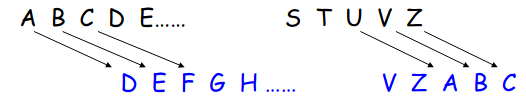
\includegraphics[width=20em]{cesare}\newline
\section{Classificazione dei cifrari}
I cifrari si dividono in:
\begin{description}
    \item[Cifrari per uso ristretto] Le funzioni C e D devono essere {\color{red}segrete}; Poco pratici per la crittografia \textit{di massa}.
    \item[Cifrari per uso generale] Si basano su un metodo a {\color{blue}chiave}. C e D sono pubbliche ma la chiave deve essere nota ai soli interessati del messaggio.
\end{description}
\subsection{Cifrari per uso generale}
Le definizioni di C e D diventano:

\begin{tabular}{l}
    C: MSG * KEYS $\rightarrow$ CRITTO\\
    D: CRITTO * KEYS $\rightarrow$ MSG\\
\end{tabular}

Se un crittoanalista entra in possesso di una chiave, basta cambiarla.
Esempi di cifrari a chiave segreta: 3DES, RC5, IDEA, AES.

\paragraph{Attacco esauriente (bruteforce)} Il crittoanalista dovrebbe provare tutte le chiavi finché non trova quella giusta per decrittare il messaggio.
Quasi impossibile da effettuare su chiavi abbastanza grandi ($>$20chars).
\section{Attacchi}
Gli attacchi possono avere successo completo (Si scopre la funzione D, compresa di chiave), oppure possono avere successo limitato (Si scopre solo qualche informazione su un messaggio).
\subsection{Attacchi al sistema crittografico}
\begin{tabular}{l | p{17em}}
    Cypher Text Attack & Il crittoanalista rileva una serie di crittogrammi $c_1, \dots, c_r$.\\
    Known Plain-Text Attack & Il crittoanalista conosce una serie di coppie $(c_1, m_1), \dots, (c_r, m_r)$.\\
    Chosen Plain-Text Attack & Il crittoanalista sceglie una serie di $m_1, \dots, m_r$ e si procura i relativi $c_1, \dots, c_m$.
\end{tabular}
\subsection{Attacchi Man-In-The-Middle MITM}
Il crittoanalista si inserisce nel canale di comunicazione e blocca tutti i messaggi diretti.
Puo' anche sostituire i messaggi originali con dei messaggi propri.
\begin{center}
    \begin{tabular}{c | c}
        Condizione normale & Attacco MITM\\
        $A \rightleftarrows B$ & $A \rightleftarrows E \rightleftarrows B$
    \end{tabular}
\end{center}

\section{Cifrari perfetti}
I cifrari perfetti sono totalmente sicuri, ma richiedono operazioni molto complesse perciò sono usati solo in condizioni estreme.
In essi $m$ e $c$ sono totalmente scorrelati tra loro.
\subsection{One-Time Pad}
E un cifrario perfetto ma ha svantaggi enormi che lo rendono quasi inutilizzabile:
\begin{itemize}
    \item Richiedono una chiave segreta nuova e perfettamente casuale per ogni messaggio.
    \item La chiave deve essere lunga quanto il messaggio.
\end{itemize}
\subsection{Cifrari sicuri}
I cifrari che vengono utilizzati ad ora non sono cifrari perfetti ma sono dichiarati sicuri. Cio' significa che non sono mai stati violati prima d'ora perché richiedono la risoluzione di problemi matematicamente difficili (Non essendo mai stato dimostrato $P \not\equiv NP$ non siamo \textit{certi} che siano inviolabili).
\section{Cifrari in uso}
\subsection{AES}
E' un \bluetext{cifrario simmetrico} (la stessa chiave viene utilizzata per crittare e decrittare), \bluetext{a blocchi} (il messaggio e' diviso in blocchi lunghi come il messaggio).
E' pubblicamente noto e utilizzato per comunicazioni \textit{non classificate}.
Si utilizzano chiavi brevi (128 o 256 bit).
\chapter{Esercizi}

\section{Correttezza RSA}

\begin{itemize}
    \item $p, q \mid m$
    \begin{itemize}
        \item Eulero: $a^{\Phi(n)} \equiv 1 \mod{n}$
        \item $e \times d \equiv 1 \mod{\Phi(n)} = 1 + r\Phi(n)$
        \item $m^{ed} \mod{n} \equiv m \times m^{r\Phi(n)} \mod{n} \equiv m \times (m^{\Phi(n)})^r \mod{n} \\\dequiv{Eul} m \times 1^r \mod{n} \equiv m \mod{n}$
    \end{itemize}
    \item $p \mid m \wedge q \nmid m$
    \begin{itemize}
        \item $m \equiv m^r \equiv 0 \mod{p} \implies (m^r - m) \equiv 0 \mod{p}$
        \item Eulero: $a^{\Phi(q)} \equiv 1 \mod{q}$
        \item $m^{ed} \mod{q} \equiv m^{1+r\Phi{n}} \mod{q} \equiv m \times m^{r(p-1)(q-1)} \mod{q} \\\equiv m \times (m^{\Phi(q)})^{r\Phi(p)} \mod{q} \equiv m \mod{q}$
        \item $(m^{ed} - m) \equiv 0 \mod{q} \implies (m^{ed} - m) \mid q$
        \item $(m^{ed} - m) \equiv 0 \mod{n} \implies m^{ed} \equiv m \mod{n}$
    \end{itemize}
\end{itemize}

\section{Cifrario perfetto}

\subsection{Definizione}

\begin{itemize}
    \item Un cifrario si dice perfetto se non \'e possibile inferire alcuna informazione sul messaggio originale, dato il crittogramma associato
    \item $\forall m \in Msg, c \in Critto, \pr(M = m) = \pr(M = m \mid C = c)$
    \item La conoscenza complessiva di un crittoanalista non cambia dopo aver letto il crittogramma in transito sul canale
\end{itemize}

\subsection{Enunciato di Shannon}

\begin{itemize}
    \item Dati $M$, l'insieme dei messaggi possibili e $K$, l'insieme delle chiavi
    \item Per Shannon : $|K| \geq |M|$
    \item Poniamo per assurdo che $|K| < |M|$
    \item Fissato un crittogramma $c \mid \pr(C = c) > 0$, esso corrisponde a $s \leq |K|$ messaggi (non necessariamente distinti) in M
    \item Dato che $s \leq |K| < |M|$ allora necessariamente esiste almeno un messaggio $m \mid \pr(M=m)>0$ non ottenibile da $c$
    \item Quindi $\pr(M=m \mid C=c) = 0 \not= \pr(M=m)$
\end{itemize}

\subsection{Perfettezza di One-Time Pad}

\begin{itemize}
    \item $\pr(M=m \mid C=c) = \dfrac{\pr(M=m,C=c)}{\pr(C=c)}$
    \item Per definizione di \m{XOR}, fissato $m$, chiavi diverse corrispondono a crittogrammi diversi
    \item Perci\`o $\pr(C = c) = (\nicefrac{1}{2})^n$ \'e costante
    \item Quindi gli eventi $(C=c) e (M=m)$ sono indipendenti
    \item Ne risulta che $\pr(M=m \mid C=c) = \dfrac{\pr(M=m) \times \cancel{\pr(C=c)}}{\cancel{\pr(C=c)}}$
\end{itemize}
\chapter{Orale}

\section{}
\chapter{Il ruolo del caso}

\section{Il significato algoritmico della casualità}

\begin{itemize}
    \item Casualità secondo Kolmogorov
    \begin{itemize}
        \item $\mathcal{K}$ : Complessità
        \item $S_i$ : Algoritmo
        \item $h$ : Sequenza "casuale"
        \item $p$ : Rappresentazione binaria dell'algoritmo
        \item $\mathcal{K}_{S_i}(h) = min\{|p| : S_i(p) = h\}$
    \end{itemize}
    \item Una sequenza \'e casuale se
    \begin{itemize}
        \item $\mathcal{K}(h) \geq |h| - \ceil{log_2(h)}$
    \end{itemize}
\end{itemize}

\subsection{Esistenza di sequenze casuali di lunghezza n}

\begin{itemize}
    \item $n$ : Lunghezza della rappresentazione binaria
    \item $S = 2^n$ : Tutte le sequenze binarie lunghe $n$
    \item Chiamiamo $T$ l'insieme delle sequenze non casuali all'interno di $S$
    \item $N = 2^{n \ceil{\log_2n} - 1}$ : Sequenze pi\'u corte di $n - \ceil{\log_2 n}$
    \item $N$ Contiene tutte anche tutti i programmi che generano le sequenze $T$
    \item $T \leq N < S$
    \item $\nicefrac{T}{S} < 2^{-\ceil{\log_2 n}}$ Tende a $0$ al crescere di $n$
\end{itemize}

\section{Generatori di numeri pseudo-casuali}

\begin{itemize}
    \item Generatore di numeri pseudo-casuali: algoritmo che parte da un piccolo valore iniziale detto seme e genera una sequenza arbitrariamente lunga di numeri.
    \item Proprietà di un generatore:
    \begin{itemize}
        \item \textbf{Frequenza} : Verifica se i diversi elementi appaiono in S approssimativamente lo stesso numero di volte
        \item \textbf{Poker} : Verifica la equidistribuzione di sottosequenze di lunghez\-za arbitraria ma prefissata
        \item \textbf{Autocorrelazione} : he verifica il numero di elementi ripetuti a distanza prefissata
        \item \textbf{Run} : verifica se le sottosequenze massimali contenenti elementi tutti uguali hanno una distribuzione esponenziale negativa
        \item \textbf{Prossimo bit} : Non esiste un algoritmo polinomiale in grado di predire l'(\textit{i} + 1)-esimo bit della sequenza conoscendo i bit precedenti
    \end{itemize} 
    \item Generatore BBS : $x_i \leftarrow (x_{i-1})^2 \text{ mod }n \wedge b_i = 1 \Leftrightarrow x_{m-i}$ e' dispari
\end{itemize}

\section{Algoritmi randomizzati}

\begin{itemize}
    \item \textit{Las Vegas} : Risultato \textbf{sicuramente} corretto in tempo \textbf{probabilmente} breve
    \item \textit{Monte Carlo} : Risultato \textbf{probabilmente} corretto in tempo \textbf{sicuramente} breve
    \item \textit{Miller e Rabin} : Algoritmo di tipo \textit{Monte Carlo} per il controllo di un numero primo
    \begin{itemize}
        \item $n$ : Valore da controllare
        \item $z$ : Intero tale che $z = \dfrac{N - 1}{2^w}$
        \item $y$ : $y \in [2, N-1]$ 
        \item P\textsubscript{1} : $mcd(N, y) = 1$
        \item P\textsubscript{2} : $(y^z \mod{N} = 1) \vee (\exists{i}, 0 \leq i \leq w-1 : y^{2^iz} \mod{N} = -1)$
        \item $(P_1 \wedge P_2) = false$ : N \'e sicuramente composto
        \item $(P_1 \wedge P_2) = true$ : N \'e primo con probabilità $p \geq \dfrac{3}{4}$
    \end{itemize}
\end{itemize}
\chapter{Esempi di algoritmi numerici}
\section{Euclide}
\[ a,b \in \mathbb{Z}, a \geq b, a > 0 \]
\begin{equation*}
    MCD(a,b) =
    \begin{cases}
        a &\text{ se } b=0\\
        MCD(b, a\Mod{b} &\text{ se } b\neq0)
    \end{cases}
\end{equation*}
Numero di passi: $O(log(a))$
\subsection{Dimostrazione}
\[ a\Mod{b} \leq \dfrac{a}{2} \]
Questo perché
\begin{equation*}
    \begin{split}
        a &\\
        & =\\
        & qb + a\Mod{b}\\
        (q = \dfrac{a}{b} \wedge a \geq b) & \geq\\
        & b + a\Mod{b}\\
        b > a\Mod{b} & >\\
        & 2a\Mod{b}
    \end{split}
\end{equation*}
Costo di MCD: $O(n^3)$
% TODO: Che cazzo e' sta roba?? ALGO di nuovo?!?
\newpage
\section{Test di primalità (inefficiente)}
\begin{algorithm*}
    \For($\sqrt{N}$: Max divisore se N non e' primo){$i=2$; $i < \sqrt{N}$; $i$++} {
        \If{$N \% i == 0$} {
            return false;
        }
    }
    return true;
    \caption{Primo(N)}
\end{algorithm*}
\chapter{Cifrari perfetti}
\section{Definizione}

\begin{itemize}
    \item $\mathcal{P}r(M = m)$ : Probabilit\'a che $m$ sia il messaggio che deve essere inviato
    \item $\mathcal{P}r(M = m \mid C = c)$ : Probabilit\'a che il messaggio originale fosse $m$ dato il crittogramma $c$ in transito
    \item Un cifrario \'e perfetto se :
    \begin{itemize}
        \item $\forall m \in \text{Msg}, c \in \text{Critto}$ : $\mathcal{P}r(M = m \mid C = c) = \mathcal{P}r(M = m)$
        \item Cio\`e $m$ e $c$ sono totalmente scorrelati tra loro perci\`o la conoscenza complessiva di un crittoanalista non cambia dopo che ha osservato un crittogramma sul canale
        \begin{itemize}
            \item In un cifrario perfetto il numero di chiavi deve essere $\geq$ dei messaggi possibili
            \item $N_m$ : Numero dei messaggi possibili
            \item $N_k$ : Numero di chiavi
            \item $N_k \geq N_m$ : Se non fosse cos\`i, dato un crittogramma $c$, esisterebbe un messaggio $m'$ non generabile tramite la decrittazione di $c$ con tutte le chiavi del sistema
            \item $\mathcal{P}r(M = m' \mid C = c) = 0 \not= \mathcal{P}r(M = m)$
        \end{itemize}
    \end{itemize}
\end{itemize}
\section{One-Time Pad}

\begin{itemize}
    \item Si assume che i messaggi $m$, le chiavi $k$, e i crittogrammi $c$ siano codificati come sequenze binarie
    \item $\mathcal{C}(m, k) = c = m \oplus k$
    \item $\mathcal{D}(c, k) = m = c \oplus k$
    \item Gen. chiave : Si costruisce una sequenza $k = k_1k_2\dots k_n : n \geq |m|$, $\mathcal{P}r(k_i = 0) = \mathcal{P}r(k_i = 1) = \nicefrac{1}{2}$
    \item Cifratura : Dati $m = m_1m_2\dots m_n$ e $k = k_1k_2\dots k_n$ $\implies$ $c = c_1c_2\dots c_n$ con $c_i = m_i \oplus k_i$
    \item Decifrazione : Identico alla cifratura ma con $c$ e $m$ invertiti
    \begin{itemize}
        \item Il cifrario One-Time Pad si considera perfetto se
        \item \textit{Tutti i messaggi hanno la stessa lunghezza n} : Altrimenti la lunghezza del crittogramma darebbe informazioni utili al crittoanalista
        \item \textit{Tutte le sequenze di $n$ bit sono messaggi possibili} : Non propriamente vero
    \end{itemize}
    \item Dimostrazione di perfezione di One-Time Pad
    \begin{itemize}
        \item $\mathcal{P}r(M = m \mid C = c) = \frac{\mathcal{P}r(M = m, C = c)}{\mathcal{P}r(C = c)}$
        \item Per definizione di \texttt{XOR} chiavi diverse generano crittogrammi diversi. Quindi fissato $m$ abbiamo $\mathcal{P}r(C = c) = (\nicefrac{1}{2})^n$ quindi gli eventi $\{M = m\}$ e $\{C = c\}$ sono indipendenti
        \item $\mathcal{P}r(M = m, C = c) = \mathcal{P}r(M = m) \times \mathcal{P}r(C = c)$
        \item $\mathcal{P}r(M = m \mid C = c) = \frac{\mathcal{P}r(M = m) \times \cancel{\mathcal{P}r(C = c)}}{\cancel{\mathcal{P}r(C = c)}} = \mathcal{P}r(M = m)$
    \end{itemize}
\end{itemize}

\section{Generazione della chiave}

\begin{itemize}
    \item Per definizione di \texttt{XOR} la chiave non pu\`o essere riutilizzata perch\`e dati
    \begin{itemize}
        \item $c' = m' \oplus k$
        \item $c'' = m'' \oplus k$
        \item $\forall i \in [0, n] \implies c'_i \oplus c''_i = m'_i \oplus m''_i$ : Cio significa che due porzioni identiche di $m'$ e $m''$ corrispondono a un tratto di $c'_i \oplus c''_i$ di tutti zeri
    \end{itemize}
    \item Metodi di generazione
    \begin{itemize}
        \item \textbf{Generatore pubblico, seme privato} : I due partner devono scambiarsi soltanto il seme ma espone il cifrario ad un attacco esauriente sui semi possibili
        \item \textbf{Generatore e seme privati} : Richiede che i partner si accordino su un generatore di loro definizione per evitare un attacco esauriente sui generatori conosciuti
    \end{itemize}
    \newpage
    \item Approssimazioni e considerazioni
    \begin{itemize}
        \item Nella realt\'a dei fatti, non tutti i $2^n$ messaggi sono messaggi possibili; Questo perch\`e si assume che il messaggio sia codificato in linguaggio naturale e deve seguire determinate regole.
        \item Nei linguaggi naturali il numero di messaggi validi di lunghezza $n$ \'e circa $\alpha^n$ con $\alpha < 2$ variabile a seconda della lingua
    \end{itemize}
\end{itemize}
\chapter{Il cifrario simmetrico standard}

\section{Criteri di Shannon}

\begin{itemize}
    \item \textbf{Diffusione} : Permutazioni ed espansioni del messaggio
    \item \textbf{Confusione} : Combinazione e compressione dei bit del messaggio e e della chiave
\end{itemize}

\section{Il cifrario DES}

\begin{itemize}
    \item Il messaggio viene diviso in blocchi da 64 bit
    \item La chiave e' composta da 8 Byte in cui ogni ottavo bit e' di parita'
    \item La cifratura e decifrazione del messaggio avviene attraverso 16 round
    \item Dalla chiave vengono create 16 sottochiavi $k[0],k[1],\dots,k[15]$ dette chiavi locali
    \item La decifrazione si esegue invertendo l'ordine delle chiavi locali
    \item Tutte le operazioni del DES sono lineari ad eccezione della S-Box
    \item Tutte le espansioni e compressioni del DES sono progettate in modo e maniera da garantire l'utilizzo di tutti i bit della chiave
\end{itemize}

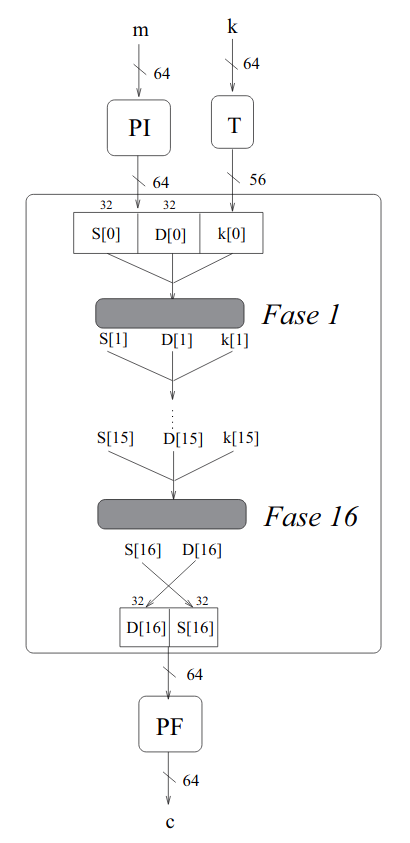
\includegraphics[width=120pt]{des1}
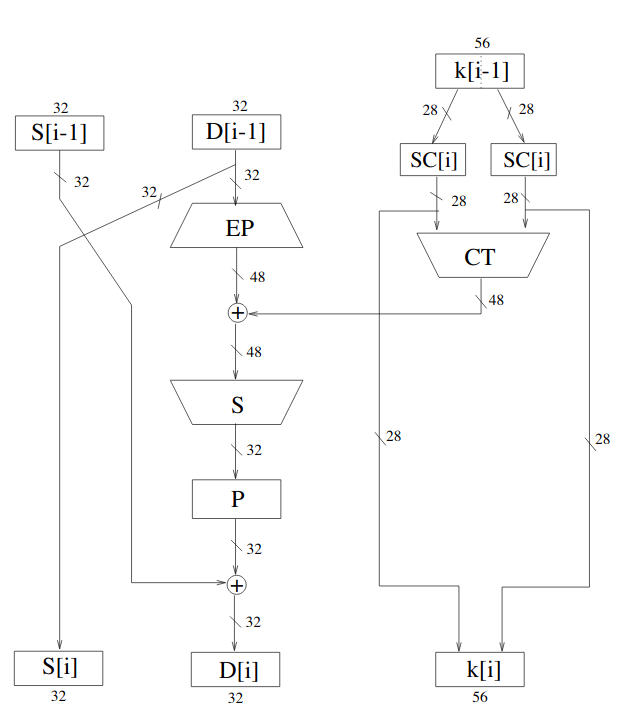
\includegraphics[width=212pt]{des2}

\subsection{Attacchi}
\begin{itemize}
    \item Proprieta' del complemento
    \begin{itemize}
        \item $\mathcal{C}_{DES}(m, k) = c \implies \mathcal{C}_{DES}(\overline{m}, \overline{k}) = \overline{c}$
        \item Procurandosi alcune coppie $\langle m, c_1 \rangle$ e $\langle \overline{m}, c_2 \rangle$ si puo' effettivamente dimezzare il numero di chiavi da testare per un attacco esaustivo
        \item Infatti se testando una chiave $k$ risulta $\mathcal{C}_{DES}(m, k) = c_1$ allora $k$ probabilmente e' la chiave
        \item Se invece risulta che  $\mathcal{C}_{DES}(m, k) = \overline{c_2}$ allora la chiave potrebbe essere $\overline{k}$
    \end{itemize}
    \item Crittoanalisi differenziale
    \begin{itemize}
        \item Si supponga di riuscire ad ottenere $2^{47}$ coppie $\langle m, c$ con $m$ scelti dal crittoanalista
        \item Si possono quindi analizzare i crittogrammi ottenuti per assegnare probabilit\'a diverse a varie chiavi
        \item La chiave originale dovrebbe quindi emergere come quella con probabilit\'a pi\'u alta
    \end{itemize}
    \newpage
    \item Crittoanalisi lineare
    \begin{itemize}
        \item Date $2^{43}$ coppie $\langle m, c \rangle$ si possono inferire alcuni bit della chiave tramite un'approssimazione lineare della funzione di cifratura e di ricavare gli altri tramite attacco esauriente
    \end{itemize}
\end{itemize}

\subsection{Variazioni del DES}

\begin{itemize}
    \item \textbf{Scelta indipendente delle sottochiavi} : Cio porta la lunghezza della chiave da 56 a 768 bit. In questo caso un attacco con analisi differenziale richiede $2^61$ coppie messaggio crittogramma
\item \textbf{3TDEA} : Si scelgono due chiavi $k_1, k_2$ e si procede come \\$\mathcal{C}_{DES}(\mathcal{D}_{DES}(\mathcal{C}_{DES}(c, k_1), k_2), k_3)$
\item \textbf{2TDEA} : Come 3TDEA con $k_3 = k_1$
\end{itemize}

\section{AES}

\begin{itemize}
    \item Cifrario simmetrico
    \item Il messaggio \'e diviso in blocchi da 128 bit
    \item Le chiavi sono da 128, 192 o 256 bit
    \item In base alla lunghezza della chiave il processo viene iterato 10 (128bit), 12 (192bit), o 14 (256bit) volte
    \item Le operazioni di ogni fase sono:
    \begin{itemize}
        \item \textbf{Op1} : Ogni Byte della matrice B \'e trasformato tramite una S-Box
        \item \textbf{Op2} : La matrice ottenuta \'e permutata tramite shift ciclici sulle righe
        \item \textbf{Op3} : Le colonne risultanti vengono trasformate tramite una operazione algebrica
        \item \textbf{Op4} : Ogni byte della matrice viene messo in \texttt{XOR} con un Byte della chiave locale per quella fase
    \end{itemize}
\end{itemize}

\section{Cifrari a composizione di blocchi}

\begin{itemize}
    \item Per la struttura dei cifrari appena descritti, blocchi identici del messaggio vengono trasformati in blocchi identici del crittogramma.
    \item Per ovviare a questo problema ci si pu\'o affidare ai cifrari a composizione di blocchi
    \item Il messaggio viene diviso in blocchi $m = m_1m_2\dots m_s$ di $b$ bit
    \item Se $m_s$ contiene $r < b$ bit lo si completa aggiungendo la sequenza $10000\dots$ di lunghezza $b - r$, altrimenti si aggiunge un nuovo blocco $m_{s+1} = 10000$
    \item Sia $c_0$ una sequenza di $b$ bit scelta in modo casuale
    \item Allora $c_i = \mathcal{C}(m_i \oplus c_{i-1}, k)$ e $m_i = c_{i-1} \oplus \mathcal{D}(c_i, k)$
\end{itemize}
\chapter{Crittografia a chiave pubblica}

\section{Funzioni One-Way Trap-Door}

\begin{itemize}
    \item Fattorizzazione
    \begin{itemize}
        \item Calcolare Il prodotto $n = pq$ e polinomialmente facile
        \item Ricavare $p$ e $q$ dato $n$ invece richiede tempo esponenziale perch\`e bisogna \textit{provarli tutti}
    \end{itemize}
    \item Calcolo della radice in modulo
    \begin{itemize}
        \item Calcolare $y = x^z \mod{s}$ richiede tempo polinomiale grazie al sistema delle successive esponenziazioni
        \item Se $s$ non \'e primo calcolare $x = \sqrt[z]{y} \mod{s}$ richiede tempo esponenziale
        \item Se per\'o $mcd(x, s) = 1$ e si conosce $v = z^{-1} \mod{\Phi(s)}$ si ha\\$y^v \mod{s} = x^{zv} \mod{s} = x^{1 + k\Phi(s)} \mod{s} = x \mod{s}$
    \end{itemize}
    \item Calcolo del logaritmo discreto
    \begin{itemize}
        \item Dati $x, y, s$ interi si richiede di trovare $z$ tale che $y = x^z \mod{s}$ 
        \item La soluzione a questo problema esiste se $s$ \'e primo e $x$ \'e un generatore di $\mathcal{Z}_s^*$
        \item Esiste un artificio piuttosto complesso per introdurre una trap-door in questa funzione
    \end{itemize}
\end{itemize}

\newpage
\section{Pregi e difetti dei cifrari a chiave pubblica}
\begin{itemize}
    \item Pregi
    \begin{itemize}
        \item Dati $n$ utenti connessi a un sistema, il numero complessivo di chiavi e' $2n$ anzich\`e $\frac{n(n-1)}{2}$
        \item Non \'e richiesto alcuno scambio segreto di chiavi
    \end{itemize}
    \item Difetti
    \begin{itemize}
        \item Il sistema \'e esposto ad attacchi di tipo \textit{chosen plain-text}
        \item Questi sistemi sono molto pi\`u lenti dei cifrari simmetrici
    \end{itemize}
\end{itemize}

\section{Il cifrario RSA}

\begin{itemize}
    \item Creazione delle chiavi
    \begin{itemize}
        \item Si scelgono $p$ e $q$ primi molto grandi
        \item $n = pq$
        \item $\Phi(n) = (p-1)(q-1)$
        \item Si sceglie $e$ : $e < \Phi(n) \wedge mcd(e, \Phi(n)) = 1$
        \item Si calcola $d = e^{-1} \mod{\Phi(n)}$ Tramite \texttt{Euclide Esteso}
        \item $k[pub] = \langle e, n \rangle$
        \item $k[prv] = \langle d \rangle$
    \end{itemize}
    \item Per cifrare un messaggio $m$ esso deve essere codificato come un intero $m < n$
    \item $m$ pu\'o essere diviso in blocchi di lunghezza $\lfloor \log_2(m) \rfloor$
    \item $c = \mathcal{C}(m, k[pub]) = m^e \mod{n}$
    \item $m = \mathcal{D}(c, k[prv]) = c^d \mod{n} = m^{ed} \mod{n} = m$
\end{itemize}

\subsection{Correttezza di RSA}

Si distinguono due casi

\begin{itemize}
    \item $p$ e $q$ non dividono $m$
    \begin{itemize}
        \item $mcd(m, n) = 1$
        \item Eulero : $m^{\Phi(n)} \equiv 1 \mod{n}$
        \item $e \times d \equiv 1 \mod{\Phi(n)} = 1 + r\Phi(n)$
        \item $m^{ed} \mod{n} = m^{1+r\Phi(n)} \mod{n} = m \times (m^{\Phi(n)})^r \mod{n} =\\\quad= m \times 1^r \mod{n} = m \mod{n}$
    \end{itemize}
    \item $m \mid p \wedge m \nmid q$
    \begin{itemize}
        \item $m \equiv m^r \equiv 0 \mod{p}, (m^r - m) \equiv 0 \mod{p}$
        \item $\Phi(q) = (q-1)$ perch\`e $q$ \'e primo
        \item $m^{\Phi(q)} \mod{q} \equiv 1 \mod{q}$
        \item $m^{ed} \mod{q} = m^{1+r\Phi(n)} \mod{q} = m \times (m^{\Phi(q)})^{r(p-1)} \mod{q} = m \mod{q}$
        \item $m^{ed} \equiv m \mod{q} \implies (m^{ed} - m) \equiv 0 \mod{q}$ : $(m^{ed} - m) \mid q$
        \item $(m^{ed} - m) \equiv 0 \mod{n} \implies m^{ed} \mod{n} = m \mod{n}$
    \end{itemize}
\end{itemize}

\section{Attacchi all'RSA}

\begin{itemize}
    \item $|p - q|$ molto piccolo
    \begin{itemize}
        \item Supponiamo $|p-q|$ piccolo
        \item $\nicefrac{p+q}{2} \approx \sqrt{n}$
        \item $\frac{(p+q)^2}{4}-n = \frac{(p-q)^2}{4}$
        \item $(\nicefrac{p+q}{2})^2 \approx n = n_a$
        \item $n_a - n = \frac{(p-q)^2}{2^2}$
        \item $\frac{(p-q)^2}{2^2} > 0 \implies n_a > n$
        \item $w = \frac{(p-q)}{2}$
        \item Bisogna trovare $z : z^2 - n = w^2$
    \end{itemize}
    \item $mcd((p-1), (q-1))$ deve essere piccolo\\(Si scelgono quindi $p$ e $q$ : $mcd(\frac{p-1}{2}, \frac{q-1}{2}) = 1$)
    \item $e = \nicefrac{1 + \Phi(n)}{k}$ con $m \mid k$ e $mcd(m, n) = 1$\\$c = m^e \mod{n} = m \times (m^{\Phi(n)})^{\nicefrac{1}{k}} \mod{n} = m \mod{n}$
    \item $e$ molto piccolo
    \begin{itemize}
        \item Poniamo che $e$ utenti condividano lo stesso valore di $e$ e che ricevano tutti lo stesso messaggio
        \item $c_i = m^e \mod{n_i}$
        \item Si assume che $n_i$ siano tutti coprimi tra loro
        \item Per \textit{Teorema Cinese del Resto}
        \begin{itemize}
            \item $n  = n_1 \times n_2 \times \dots \times n_e$
            \item $m' < n$
            \item $m' \equiv m^e \mod{n}$
        \end{itemize}
        \item $m^e$ {\tiny($\equiv m'$)} $< n$
        \item $m' = m^e$ : Perch\`e $m'$ e $m^e$ sono minori di $n$
        \item $m = \sqrt[e]{m'}$
        \item Per mantenere valori di $e$ piccoli senza compromettere la sicurezza basta aggiungere una sequenza di bit diversa alla fine di ogni messaggio (\textit{padding})
    \end{itemize}
    \item $n$ uguale per pi\'u utenti
    \begin{itemize}
        \item Date due chiavi $\abracket{e_1, n}, \abracket{e_2, n} : mcd(e_1, e_2) = 1$
        \item Tramite \texttt{Euclide Esteso} si possono calcolare $r$ e $s$ tali che $e_1r + e_2s = 1$ (Fissiamo $r < 0$)
        \item Poniamo adesso che si intercettino due crittogrammi $c_1, c_2$ relativi allo stesso messaggio $m$ diretti ai due utenti attaccati
        \item $m = m^{e_1r+e_2s} = (c_1^r \times c_2^s) \mod{n} = ((c_1^{-1})^{-r} \times c_2^s) \mod{n}$
        \item Tramite \texttt{Euclide Esteso} si calcola $c^{-1} \mod{n}$
        \item Si pu\'o quindi calcola $m$ in tempo polinomiale
    \end{itemize}
    \item RSA ha gli stessi problemi (e le stesse soluzioni) del DES per la periodicit\'a dei blocchi 
\end{itemize}

\section{Diffie-Hellman per lo scambio di chiavi}

\begin{itemize}
    \item A e B si accordano su un primo $p$ e un generatore $g$ di $\mathcal{Z}_p^*$
    \item A sceglie $x < p$ casuale e calcola $X = g^x \mod{p}$ e spedisce $X$ a B
    \item B fa lo stesso ($Y = g^y \mod{p}$)
    \item Entrambi calcolano $k[session] = Y^x \mod{p} = X^y \mod{p} =\\= g^{xy} \mod{p}$
    \item Se un crittoanalista intercetta $X$ (o $Y$) dovrebbe calcolarsi il logaritmo discreto per risalire a $x$ (o $y$)
    \item L'unico attacco possibile \'e \texttt{MITM}
\end{itemize}

\section{Curve ellittiche su campi finiti}

\begin{itemize}
    \item $E_p(a, b) = \{(x, y) \in \mathcal{Z}_p^2 \mid y^2 \mod{p} = (x^3 + ax + b) \mod{p}\} \cup \{O\}$
    \item La curva presenta una simmetria rispetto alla retta $y = p/2$
\end{itemize}
% TODO

\section{Diffie-Hellman su curve ellittiche}

\begin{itemize}
    \item A e C si accordano su una curva definita su campo finito, e su un punto $B$ di ordine $n$ molto grande
    \item $n$ \'e il pi\'u piccolo intero tale che $nB = O$
    \item A sceglie un intero $n_A < n$ e genera $P_A = n_AB$ e invia $P_A$ a C
    \item C fa lo stesso ($P_C = n_CB$)
    \item Entrambi calcolano $S = n_AP_C = n_cP_A = n_An_CB$
    \item $k = x_S \mod{2^{256}}$
\end{itemize}

\section{Algoritmo di Koblitz}

Questo algoritmo serve a trasformare un messaggio $m < p$ in un punto $P_m$ della curva $E_p(a, b)$
\begin{itemize}
    \item Si fissa $h \mid (m+1)h < p$
    \item Si prova ogni $i \in [0, h)$ si calcola $x_i = mh + i$
    \item Se esiste la radice quadrata di $y_i^2 = x_i^3 + ax_i + b$ allora si sceglie $P_m = (x_i, y_i)$, altrimenti si itera la $i$
\end{itemize}

Questo algoritmo ha probabilit\'a di successo pari a $1-\nicefrac{1}{2^h}$

\section{Algoritmo di ElGamal su curve ellittiche}

\subsection{Cifratura}

\begin{itemize}
    \item M sceglie $r$ casuale
    \item $V = rB$
    \item $W = P_m + rP_D$ dove $P_D$ \'e la chiave pubblica di D
    \item Invia $\abracket{V,W}$
\end{itemize}
\subsection{Decifrazione}
\begin{itemize}
    \item Calcola $P_m = W - n_DV = P_m + rP_D - n_D(rB) =\\= P_m + \cancel{r(n_DB)} - \cancel{n_DrB}$
\end{itemize}

\section{Sicurezza della crittografia su curve ellittiche}

\begin{itemize}
    \item Per calcolare il logaritmo discreto in algebra modulare e la fattorizzazione degli interi esiste un algoritmo sub-esponenziale chiamato \textit{index calculus}
    \item Questo algoritmo richiede in media $O(2^{\sqrt{b \log b}})$ operazioni per chiavi di $b$ bit
    \item Per il problema del logaritmo discreto su curve ellittiche invece non esiste un algoritmo del genere
    \item L'algoritmo pi\`u efficiente conosciuto ad oggi ($Pollard\ \rho$) richiede in media $O(2^{b/2})$ operazioni quindi \'e pienamente esponenziale
\end{itemize}

\begin{center}
    \begin{tabular}{|c|c|c|}
        \hline
        TDEA, AES & RSA e DH & ECC\\
        (bit della chiave) & (bit del modulo) & (bit dell'ordine)\\
        \hline
        80 & 1024 & 160\\
        112 & 2048 & 224\\
        128 & 3072 & 256\\
        192 & 7680 & 384\\
        256 & 15360 & 512\\
        \hline
    \end{tabular}
\end{center}
\chapter{La firma digitale}

Ai protocolli crittografici sono richieste tre funzionalit\'a importanti

\begin{itemize}
    \item Identificazione : Un sistema deve essere in grado di accertare l'identit\'a di un utente che richiede di accedere ai suoi servizi
    \item Autenticazione : Il destinatario di un messaggio deve essere in grado di accertare l'identit\'a del mittente e l'integrit\'a di un crittogramma ricevuto
    \item Firma digitale : Come una firma manuale, deve possedere tre caratteristiche (accertabili anche da una terza parte facente da giudice)
    \begin{itemize}
        \item Il mittente non ha facolt\'a di ripudiare il messaggio
        \item Il destinatario deve poter accertare l'identit\'a del mittente e l'integrit\'a del crittogramma
        \item Il destinatario non deve poter sostenere che $m' \not= m$ \'e il messaggio inviatogli
    \end{itemize}
\end{itemize}

\section{Funzioni hash one-way}

\begin{itemize}
    \item Una funzione hash $f : X \to Y$ \'e definita per $n = |X| \gg m = |Y|$
    \item La differenza di cardinalit\'a tra $X$ e $Y$ implica che esiste una partizione di $X$ in sottoinsiemi disgiunti $X_1,\dots,X_m \mid \forall i \in [1,m]$ tutti gli elementi in $X_i$ hanno come immagine uno stesso elemento in $Y$
    \item Una funzion hash one-way deve soddisfare tre caratteristiche
    \begin{itemize}
        \item Per ogni $x \in X$ \'e computazionalmente facile calcolare $f(x)$
        \item Per la maggior parte degli $y \in Y$ \'e computazionalmente difficile determinare $x$ tale che $f(x) = y$ (one way)
        \item \'E computazionalmente difficile determinare una coppia $x', x''$ in $X$ tale che $f(x') = f(x'')$ (claw free)
    \end{itemize}
\end{itemize}

\section{Identificazione}

\begin{itemize}
    \item Le password in un database vengono salvate sotto forma di hash con il seguente meccanismo
    \item Durante la fase di registrazione un utente sceglie una password $P_u$
    \item Il sistema genera un seme $S_u$ e calcola un hash $Q_u = f(P_uS_u)$ e memorizza $\abracket{u, S_u, Q_u}$
    \item Quando un utente prova ad effettuare l'accesso, il sistema recupera il suo seme e calcola $Q'_u$
    \item Se $Q'_u = Q_u$ l'identificazione ha avuto successo
    \item Alla password viene aggiunto un seme perch\`e altrimenti password uguali genererebbero hash uguali
\end{itemize}

\subsection{Identificazione tramite RSA}

\begin{itemize}
    \item Il sistema $S$ genera un valore casuale $r < n$ e lo invia in chiaro a $U$
    \item $U$ applica la sua chiave privata r calcolando $f = r^d \mod{n}$
    \item $S$ verifica l'identit\'a di $U$ applicando la chiave pubblica di $U$ stesso verificando che $f^e \mod{n} = r$
\end{itemize}

Questo protocollo per\`o richiede che $U$ si fidi di $S$. Infatti se $S$ non fosse \textit{chi dice di essere}, potrebbe richiedere a $U$ di applicare la propria chiave privata a messaggi opportunamente creati per inferire informazioni su $d$

\section{Autenticazione}

\begin{itemize}
    \item Il meccanismo di autenticazione pu\'o essere descritto attraverso una funzione $\mathcal{A}(m, k)$ che genera un'informazione (detta MAC) utile a garantire la provenienza e l'integrit\'a di m
    \item Se non \'e richiesta la confidenzialit\'a, \texttt{Mitt} spedisce la coppia\\$\abracket{m, \mathcal{A}(m, k)}$
    \item Altrimenti spedisce la coppia $\abracket{\mathcal{C}(m, k'), \mathcal{A}(m, k)}$
    \item Si pu\`o generare un MAC tramite una funzione hash one-way concatenando il messaggio e la chiave
    \item $\mathcal{A}(m, k) = h(mk)$
\end{itemize}

\section{Firma digitale}

\subsection{Messaggio cifrato e firmato in hash}

\begin{itemize}
    \item Il mittente $U$ calcola $f = \mathcal{D}(h(m), k_U[prv])$ e $c = \mathcal{C}(m, k_V[pub])$
    \item Spedisce la tripla $\abracket{U, c, f}$ a $V$
    \item $V$ calcola $m = \mathcal{D}(c, k_V)[prv]$ e $h(m) = \mathcal{C}(f, k_U[pub])$
    \item Se $h(m)$ \'e uguale al valore ottenibile ricalcolando la funzione hash sul messaggio, la firma \'e valida
\end{itemize}

\section{La Certification Authority}

\begin{itemize}
    \item Le \m{CA} autenticano le associazioni $\langle$ \m{utente, chiave pubblica} $\rangle$
    \item Un certificato contiene la chiave pubblica e una lista di informazioni relative al suo proprietario, tutto opportunamente firmato dalla \m{CA}
    \item Se \m{U} vuole comunicare con \m{V}, richiede cert$_V$ alla \m{CA}
\end{itemize}

\subsection{Messaggio cifrato, firmato in hash, e certificato}

\begin{itemize}
    \item \m{U} calcola $f$ e $c$ come nel protocollo senza certificato
    \item Spedisce la tripla $\abracket{cert_U, c, f}$
    \item \m{U} verifica $cert_U$ con la sua copia della chiave pubblica della \m{CA}
    \item Procede cone nel protocollo senza certificato
\end{itemize}

\section{Il protocollo SSL}

\section{Protocolli Zero-Knowledge}

\begin{itemize}
    \item Nei protocolli Zero-Knowledge due entit\'a (Prover $P$ e Verifier $V$) non si fidano l'uno dell'altro
    \item Il prover dovr\'a essere in grado di dimostrare al Verifier di essere in possesso di una facolt\'a particolare senza comunicargli alcuna informazione su di essa
    \item Questi protocolli si basano su una serie di iterazioni, dopo ognuna delle quali in Verifier aumenta la sua confidenza che $P$ sia \textit{chi dice di essere}
\end{itemize}

\end{document}